\documentclass[fontsize=10pt,paper=a4,open=any,
twoside=no,toc=listof,toc=bibliography,headings=optiontohead,
captions=nooneline,captions=tableabove,english,DIV=15,numbers=noenddot,final,parskip=half-,
headinclude=true,footinclude=false,BCOR=0mm]{scrartcl}
\pdfvariable suppressoptionalinfo 512\relax
\synctex=1

\author{Valentin Boettcher}
\usepackage{hirostyle}
\usepackage{hiromacros}
\addbibresource{references.bib}
\acsetup{
  make-links = true ,
  format = \emph ,
  list / display = all ,
  pages / display = all
}
\DeclareAcronym{mlong}{short=LTAD, long=long-time time-averaged mean displacement}
\DeclareAcronym{rwa}{short=RWA, long=Rotating-Wave Approximation}

\title{The non-Markovian Quantum Walk for Finite Baths}
\date{2023}
\graphicspath{{plots}}

\begin{document}
\maketitle
\tableofcontents

We will discuss how the behavior of the model introduced in
\refcite{Ricottone2020} for the limit of weak coupling and an infinite
bath may be reproduced with both finite coupling strength and a finite
number of bath levels.

The model Hamiltonian is that of an SSH-Chain~\cite{Su1979} with a
number of bath states coupled to each unit cell \(H=H_{A}+H_{\bar{A}}+V\)
\begin{align}
  \label{eq:36}
  H_{A} &= ∑_{m}ω_{A} \ketbra{A,m} \\
  H_{\bar{A}} &= Σ_{m}(ω_{A} + ω)\ketbra{B,m}+
                   ∑_{j}\bqty{ω_{j}\ketbra{j, k} + g_{j}
                   \pqty{\ketbra{j,m}{B,m} + \hc}}\\
  V&=∑_{m} v\pqty{\ketbra{A,m}{B,m} + u\ketbra{A,m}{B,m+1} + \hc}
\end{align}

In momentum space, the model Hamiltonian takes the form \(H=H_{A}(k) +
H_{\bar{A}}(k) + V(k)\) with
\begin{align}
  \label{eq:35}
  H_{A}(k) &= ω_{A} \ketbra{A,k} \\
  H_{\bar{A}}(k) &= (ω_{A} + ω)\ketbra{B,k}+
                   ∑_{j}\bqty{ω_{j}\ketbra{j, k} + g_{j}
                   \pqty{\ketbra{j,k}{B,k} + \hc}}\\
  V(k)&=\abs{v(k)}\pqty{\eu^{\iu ϕ(k)}\ketbra{A,k}{B,k} + \hc}
\end{align}
with \(v(k) = \abs{v (1+u\eu^{\iu k})}\).

Upon eliminating the \(B\) site from the above through a
Schrieffer-Wolff transformation for \(ω\gg v(k)\), we end up with
\begin{equation}
  \label{eq:37}
  H(k) = \tilde{ω}_{A} \ketbra{j,k} + ∑_{j} \bqty{\tilde{ω}_{j} \ketbra{j, k}
    + \pqty{\tilde{η}_{j}\ketbra{A,k}{j,k} + \hc}},
\end{equation}
where the \(\tilde{η}_{j}(k) \sim \tilde{η}_{j}(0) v(k)\). The tildas
signify quantities renormalized due to the Schrieffer-Wolff transform
and will be dropped in the following.


The \emph{mean displacement} is defined as
\begin{equation}
  \label{eq:38}
  \ev{m(t)} \equiv ∑_{m}m \pqty{1-ρ_{A,m}}  = ∑_{m}m \pqty{1-\abs{\braket{A,m}{ψ(t)}}^{2}}
\end{equation}
where we consider the initial condition \(\ket{ψ(0)}=\ket{A,0}\) and
define \(ρ_{A}(t)=\abs{\braket{A,m}{ψ(t)}}^{2}\) for convenience.

As the quantity \(\ev{m(t)}\) can fluctuate in time and we will be
interested in long-time beahavior, we additionally define
\begin{equation}
  \label{eq:39}
  \ev{m} \equiv \lim_{T\to ∞} \frac{1}{T}∫_{0}^{T}\ev{m(t)} \dd{t}
\end{equation}
which we will refer to as \ac{mlong}.

In momentum space this becomes
\begin{equation}
  \label{eq:40}
  \ev{m} = ∫_{0}^{2π}(1-ρ_{A})\pdv{ϕ(k)}{k} \frac{\dd{k}}{2π}
\end{equation}
with
\begin{equation}
  \label{eq:41}
  ρ_{A}(k) = \lim_{T\to ∞}\frac{1}{T} ∫_{0}^{T}ρ_{A}(t, k)\dd{t} = \lim_{T\to
    ∞}\frac{1}{T} ∫_{0}^{T}\abs{\braket{A,k}{ψ(t)}}^{2}\dd{t}.
\end{equation}

\section{Born Approximation}
\label{sec:born-approximation}

In the limit of very weak coupling we can solve for \(ρ_{A}\) in terms
of a non-Markovian master equation by employing perturbation theory to
second order\footnote{Which is the first nontrivial order} in the
coupling \(V\).
\begin{equation}
  \label{eq:42}
  \dot{ρ}_{A}(k,t) = ∫_{0}^{t}Σ(k, t-t\prime) ρ_{A}(k, t\prime)
\end{equation}
with the self-energy
\begin{equation}
  \label{eq:43}
  Σ(k,t)=-2 ∑_{j}\abs{η_{j}(k)}^{2}\cos((ω_{k}-ω_{A})t)
\end{equation}
with \(j=\overline{1,N}\).

We are interested in the long time average of \(ρ\) which can be
expressed as
\begin{equation}
  \label{eq:44}
  {ρ}_{A}(k)=\lim_{T\to
    ∞}\frac{1}{T}∫_{0}^{∞}\eu^{-\frac{t}{T}}ρ_{A}(k,t)\dd{t} =
  \lim_{s\to 0} s \tilde{ρ}_{A}(k, s) = \eval{\bqty{\dv{s} \frac{1}{\tilde{ρ}_{A}(k,s)}}^{-1}}_{s=0}
\end{equation}
where \(\tilde{ρ}_{A}({k, s})\) is the Laplace transform of \(ρ_{A}(k,
t)\).

The equation of motion \cref{eq:42} gives direct access to
\(\tilde{ρ}_{A}\)
\begin{equation}
  \label{eq:45}
  \tilde{ρ}_{A}({k, s}) = \frac{ρ_{A}(k,0)}{s - \tilde{Σ}(k, s)} = \frac{1}{s - \tilde{Σ}(k, s)},
\end{equation}
with
\begin{equation}
  \label{eq:46}
  \tilde{Σ}(k, s) = -2 ∑_{j}\abs{η_{j}}^{2} \frac{s}{s^{2}+(ω_{j}-ω_{A})^{2}} =
  -∑_{j}\abs{η_{j}}^{2} \bqty{\frac{1}{s+\iu (ω_{j}-ω_{A})} + \frac{1}{s-\iu
      (ω_{j}-ω_{A})}}.
\end{equation}

Using \cref{eq:44} and setting \(ω_{A}=0\), this yields
\begin{equation}
  \label{eq:47}
  ρ_{A}(k) = \frac{1}{1 + 2∑_{j}\frac{\abs{η_{j}}^{2}}{ω_{j}^{2}}} =
  \frac{1}{1+2 U_{A}}.
\end{equation}

We now assume that the \(η_{j}\) are chosen so that in the continuum
limit \(N\to ∞\)
\begin{equation}
  \label{eq:48}
  ∫_{0}^{∞}f(ω)∑_{j}\abs{η_{j}}^{2} δ(ω-ω_{j})^{2}\dd{ω} =
  ∫_{0}^{∞}J(ω) f(ω)
\end{equation}
for arbitrary (smooth) functions \(f\), where \(J\) is called the
spectral density. We make the model assumption
of an ohmic-type spectral density
\begin{equation}
  \label{eq:49}
  J(ω) =g_{0}^{2}\frac{α+1}{ω_{c}^{α+1}}
  \begin{dcases}
    ω^{α} & \mathrm{if}\, ω \leq ω_{c},\\
    0 & \mathrm{otherwise}.
  \end{dcases}
\end{equation}
For \(α<(>)1\) this we call \(J\) a sub(super)-Ohmic spectral density,
whereas for \(α=1\) we have an Ohmic spectral density. Let us define
\(J_{α}=g_{0}^{2}\frac{α+1}{ω_{c}^{α+1}}\) for convenience.


The \(ω_{j}\) and \(η_{j}\) may be chosen according to
\cref{sec:discretization-bath}.

In the continuum limit \(U_{A}\to ∞\) for \(α\leq 1\) and remains finite
for \(α>1\), which leads to the \ac{mlong} \(\ev{m}\) having a sharp
transition from \(0\) to \(1\) for \(α\leq 1\) which becomes washed
out for \(α>1\).

We wish to study how this limit is approached with a finite bath and
in finite times. The born approximation requires that \(η\to 0\)
sufficiently fast for \(N\to ∞\) so that the resulting long timescale is
unlikely to be resolved experimentally.

\section{Exact Solution}
\label{sec:exact-solution}

Numerics (see \cref{fig:unshifted_overview}) at finite coupling
strengths suggest that the behavior for the weak coupling limit may
not be naively reproduced in this setting.

\begin{figure}[htp]
  \centering
  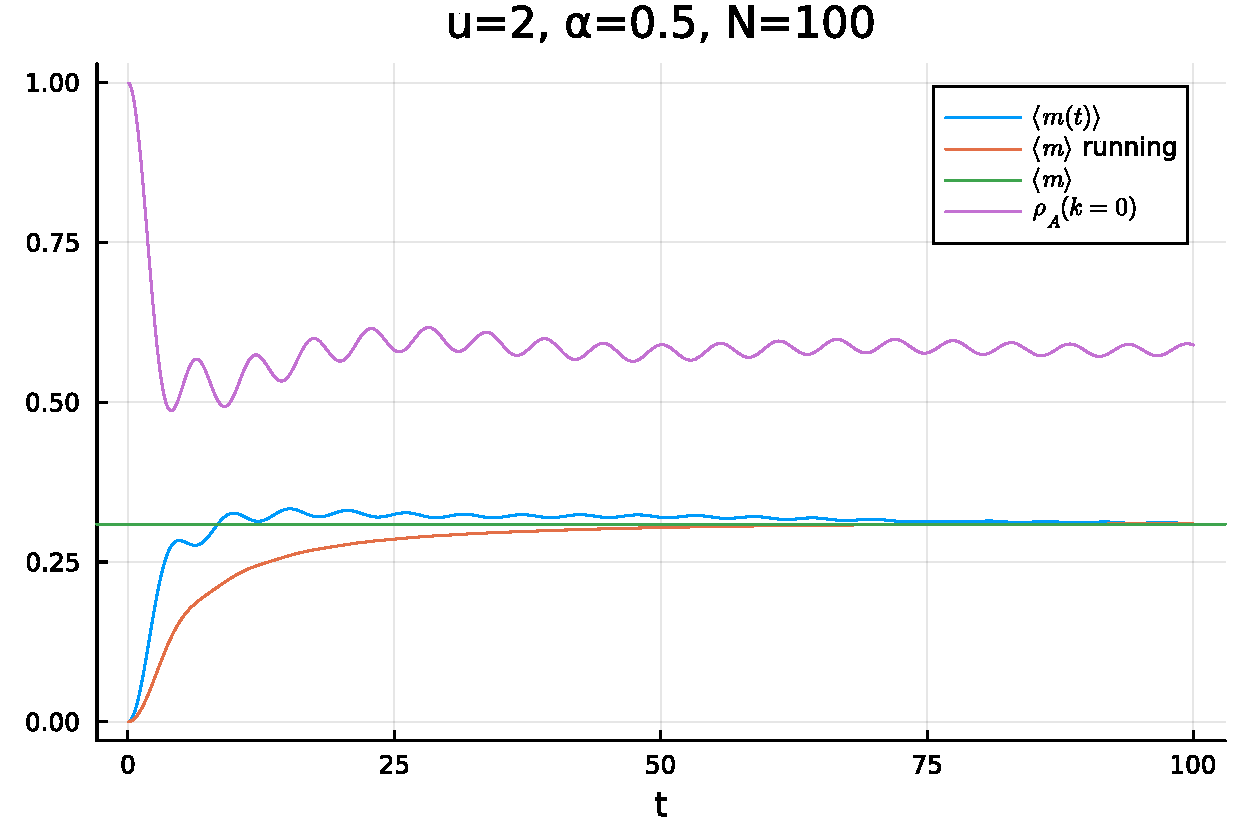
\includegraphics[width=.8\linewidth]{plots/overview_unshifted.tikz}
  \caption{\label{fig:unshifted_overview} A numerical simulation for
    \(g_{0}=10^{-2}\). The mean displacement takes on some
    non-universal value and \(ρ_{A}\not{\to} 0\).}
\end{figure}

In the following we will suppress the \(k\) dependence of the
couplings \(η_{j}\).  Perturbation theory suggests that the energy of
the \(\ket{A}\) state changes according to a lamb shift
\begin{equation}
  \label{eq:1}
  ω_{A} \to ε_{A}^{(2)} = ω_{A} - ∑_{j} \frac{\abs{η_{j}}^{2}}{(ω_{j}-ω_{A})},
\end{equation}
which would make the system insensitive to the spectral density at
\(ω = 0\) unless corrected for.

Let us proceed by writing down the equations of motion for the
coefficients of a general state \(\ket{ψ} = α\ket{A} +
∑_{j}β_{j}\ket{j}\) following from \cref{eq:37}
\begin{equation}
  \label{eq:2}
  \begin{aligned}
    \iu \dot{α} &= ω_{A}α + ∑_{j} η_{j} β_{j} & \iu \dot{β}_{j} = η_{j}^\ast α
                                       + ω_{i} β_{i}.
  \end{aligned}
\end{equation}
Transforming the \(β_{j}\) into a rotating frame with respect to the
\(ω_{i\neq A}\) so that \(\tilde{β}_{i}=β_{i} \eu^{\iu ω_{i}t}\) we obtain
\begin{equation}
  \label{eq:3}
  \begin{aligned}
    \iu \dot{α} &= ω_{A}α + ∑_{j} η_{j} \tilde{β}_{j}\eu^{-\iu ω_{j}t}
    & \iu \dot{\tilde{β}}_{j} = η_{j}^\ast α \eu^{\iu ω_{j} t}.
  \end{aligned}
\end{equation}

The equations for the \(\tilde{β}_{j}\) can be integrated straight forwardly
to obtain \(\tilde{\beta}_{j} = -\iu η_{j}^{\ast} ∫_{0}^{t}\eu^{\iu ω_{i} τ}
  α(τ) \dd{τ}\) which can be substituted into \cref{eq:3} to find a
  closed equation for \(α\)
\begin{equation}
  \label{eq:4}
  \dot{α} = -\iu ω_{A}α - ∫_{0}^{t} Κ(t-τ)α(τ) \dd{τ}
\end{equation}
with \(Κ(t-τ) = ∑_{j} \abs{η_{j}}^{2} \eu^{-\iu ω_{i}
  (t-τ)}\). Laplace transforming both sides of \cref{eq:4} leads us to
\begin{equation}
  \label{eq:5}
  \begin{aligned}
  \tilde{α}(s) &= \frac{α(0)}{s+\iu ω_{A} + \tilde{Κ}(s)} &
     \tilde{Κ}(s) &= ∑_{j}\frac{\abs{η_{j}}^{2}}{s + \iu ω_{j}},
  \end{aligned}
\end{equation}
which is very similar to \cref{eq:45}, save for the explicit
appearance of \(\iu ω_A\). As \cref{eq:45} is related to a probability, it
is real-valued and always has a pole at \(s=0\) independent of
\(ω_{A}\).

The amplitude \(α\) on the other hand can generically be expected to
have the form \(α(t)=∑_{i}α_{i}\eu^{-\iu ε_{i} t}\), where the
\(ε_{i}\) are poles of \(\tilde{α}(s)\) and
\begin{equation}
  \label{eq:6}
  α_{i} = \iu \lim_{ε\to ε_{i}} (ε-ε_{i}) \tilde{α}(-\iu ε) =
  \eval{\bqty{\dv{s} \frac{1}{\tilde{α}(-\iu s)}}^{-1}}_{s=ε_{i}} =
  \frac{α(0)}{1 + \tilde{Κ}'(-\iu ε_{i})} = \frac{α(0)}{1+U_{i}}
\end{equation}
are the residues (modulo \(2π\iu\)) of \(\tilde{α}(s)\).

We are however interested in the behaviour of \(ρ_{A}(t) =
\abs{α(t)}^{2} = ∑_{jk}α_{j}α_{k}^\ast \eu^{-\iu (ε_{j} - ε_{k})t}\)
which has the long time average \(ρ_{A} = ∑_{j}
\abs{α_{j}}^{2}\). Therefore we cannot simply calculate the residue at
\(s=0\) as in \cref{sec:born-approximation}, but have to
calculate all \(α_{j}\) in principle.

Again, perturbation theory suggests, that there will be one eigenstate
with great overlap with the \(\ket{A}\) state, close in energy to
\(ω_{A}\). Let us designate the corresponding residual as \(α_{A}\)
and notice that \(\abs{α_{A}}\) forms a lower bound of
\(ρ_{A}(t)\). We can therefore expect that for relatively weak
coupling (which we will make more concrete later), the \(α_{A}\) can
be viewed as a good approximation for \(ρ_{A}\) and as an indicator
for \(ρ_{A}(t) \not\to 0\) in general.

Finding the pole of \(\tilde{α}(s)\), or equivalently the root of
\({s+\iu ω_{A} + \tilde{Κ}(s)}\) close to \(-\iu ω_{A}\) involves
finding the root of a polynomial of potentially high degree and can in
general only be achieved through numerics or perturbation
theory. Further, \cref{fig:unshifted_overview} suggests that we won't
obtain a results similar to the one found in
\cref{sec:born-approximation}.

The solution is to demand the existence of a pole at \(s=0\)
corresponding to \(ε_{A}=0\) and adjusting \(ω_{A}\) accordingly
\begin{equation}
  \label{eq:7}
  0 = \iu ω_{A} + \tilde{Κ}(0) \implies ω_{A} = ∑_{j}\frac{\abs{η_{j}}^{2}}{ε_{j}}
\end{equation}
which is only consistent with the expression obtained using
second-order perturbation theory\footnote{and therefore the Born
  approximation in the current context} \cref{eq:7} only for
\(∑_{j}{\abs{η_{j}}^{2}}/{ω_{j}^{2}}\ll 1\) and \(\abs{ω_{A}} \ll ω_{j}\).

Using \cref{eq:6,eq:7} and we can conclude that
\begin{equation}
  \label{eq:8}
  U_{A} = ∑_{j}\frac{\abs{η_{j}}^{2}}{ω_{j}^{2}} \implies ρ_{A}≥ \abs{α_{A}}^{2}
  = \frac{α(0)}{(1+U_{A})^{2}},
\end{equation}
which is compatible with \cref{eq:47} for \(U_{A}\ll 1\) as already
stated in the previous paragraph.

It is to be stressed, that \cref{eq:8} is an exact result and exhibits
the same behavior as the result from \cref{sec:born-approximation}, as
the values for \(U_{A}\) obtained are identical. On the other hand, we
are interested in the case where \(U_{A}\to ∞\) where the
compatibility with the Born approximation should be broken. One could
however imagine, that there is the possibility of \(U_{A}\gg 1\) while
\(ω_{A}\ll ω_{c} \implies ε_{A}^{(2)}\approx ε_{A} \approx 0\) so that
the two methods converge again at sufficiently low coupling strength
and large bath size.

% This can, in fact, be achieved. Consider the first bath level to have
% energy \(ω_{1} = ε\). According to \cref{sec:discretization-bath}, we
% can assign it a coupling
% \(η_{j}^{2} = ∫_{0}^{ε}J(ω)\dd{ω} \approx J(ε/2)ε\). Considering only
% this first bath mode, as it is going to have the greatest influence in
% the sums above for \(ε\ll ω_{c}\) (\(N\to ∞\)) and
% \(g_{0}\ll ω_{c}^{2}\), we can approximate
% \begin{equation}
%   \label{eq:9}
%   \begin{aligned}
%   \frac{ω_{A}}{ω_{c}} &\sim \frac{g_{0}^{2}(α+1)}{ω_{c}^{α+2} 2^{α}} ε^{α} & U_{A}
%     &\sim  \frac{g_{0}^{2}(α+1)}{ω_{c}^{α+1} 2^{α}} ε^{α-1}.
%   \end{aligned}
% \end{equation}
% When \(α<1\), we have \({ω_{A}}/{ω_{c}}\to 0\) while \(U_{A}\to ∞\)
% for \(ε\to 0\)
% fulfilling \cref{eq:1} as well as \cref{eq:7}.

However, in the continuum limit
\begin{equation}
  \label{eq:10}
  ω_{A} = ∫_{0}^{ω_{c}}\frac{J(ω)}{ω} = J_{α}\frac{ω_{c}^{α}}{α}.
\end{equation}
Using this in \cref{eq:46} and taking the limit \(g_{0}\to 0\) leads
to \(ρ_{A}\to 1\), whereas \cref{eq:8} would suggest \(ρ_{A}\to
0\). Therefore the weak coupling limit has to be taken at the same
time as the continuum limit to achieve consistency. \emph{I have to
  think more about that.} This is sensible, as the transition
\(U_{A}\to ∞\) may well be non-analytic in \(g_{0}\).

\subsection{Strong Coupling Limit}
\label{sec:strong-coupl-limit}

In the strong coupling limit
\begin{equation}
  \label{eq:14}
  ∑_{j}\abs{η_{j}}^{2} \gg ω_{c}^{2}
\end{equation}
we can find an effective two-level system behavior in the model
\cref{eq:37}.

Starting from the eigenvalue equations
\begin{align}
  \label{eq:11}
    ω_{A} α + ∑_{j} η_{j} β_{j} &= E α \\
    ω_{j} β_{j} + η_{j} α &= E β_{j} \label{eq:12}
\end{align}
and substituting \cref{eq:12} into \cref{eq:11} to obtain
\begin{equation}
  \label{eq:12}
  E = ω_{A} + Σ(E) = ω_{A} + ∑_{j}\frac{\abs{η_{j}}^{2}}{E-ω_{j}}
\end{equation}
which should be familiar from \cref{eq:5}. We can now expect some
energy eigenvalues \(E\) close to the bath energies \(ω_{j}\), but
level repulsion will produce states with a large overlap with
\(\ket{A}\) that have energies outside of this ``continuum'' as is
demonstrated in \cref{fig:spectrum_strong_coupling_limit}.
\begin{figure}[htp]
  \centering
  \includegraphics[width=.49\linewidth]{plots/spectrum_weak_couplign_limit.tikz}
  \includegraphics[width=.49\linewidth]{plots/spectrum_stong_couplign_limit.tikz}
  \caption{\label{fig:spectrum_strong_coupling_limit} The spectrum of
    the model in \cref{fig:unshifted_overview} for two different
    coupling strengths. The bars show the overlap
    \(\abs{\braket{A}{E}}^{2}\) of the eigenstate \(\ket{E}\) at
    energy \(E\) with the \(\ket{A}\) state.}
\end{figure}

Assuming \(\abs{E}\gg ω_{c} \implies \abs{E} \gg ω_{j}\) we can
neglect the \(ω_{j}\) in \cref{eq:12} to obtain
\begin{equation}
  \label{eq:13}
  E_{\pm} = \frac{1}{2}\bqty{ω_{A}\pm \sqrt{ω_{A}^{2} + 4 ∑_{k}\abs{η_{j}}^{2}}}.
\end{equation}
For \(ω_{A} = 0\) this becomes \(E_{\pm}=\pm\sqrt{∑_{j}\abs{η_{j}}^{2}}\) which
leads to the criterion \cref{eq:14}.

The corresponding eigenvectors are (modulo normalization)
\begin{equation}
  \label{eq:15}
  \ket{\pm} = \frac{1}{\sqrt{1 + ∑_{j}
      \abs{\frac{η_{j}}{E_{\pm}-ω_{j}}}^{2}}}\bqty{\ket{A} +
    ∑_{j} \frac{η_{j}^\ast}{E_{\pm}-ω_{j}}\ket{j}}\approx \frac{1}{\sqrt{2}}\bqty{\ket{A} +
    ∑_{j} \frac{η_{j}^\ast}{E_{\pm}}\ket{j}}
\end{equation}
where the second approximate equality follows from
\(\abs{E}\gg \abs{ω_{A}}\). Together they form a complete orthonormal
basis of the subspace of the Eigenspace of the Hamiltonian that
contains \(\ket{A}\) of the equal overlap with \(\ket{A}\).

A state \(\ket{ψ(t)}\) with
\(\ket{ψ(0)}=\ket{A} = (\ket{+} + \ket{-})/\sqrt{2}\) will oscillate
between \((\ket{+} \pm \ket{-})/\sqrt{2}\) with angular frequency
\(2\abs{E_{\pm}}\) and thus
\(ρ_{A}(k,t)=\cos[2](E_{+}t)=\cos[2](E_{-}t) \implies ρ_{A}(k) =
1/2\). The \ac{mlong} will then exhibit a universal behavior
irrespective of the spectral density
\begin{equation}
  \label{eq:16}
  \ev{m} =
  \begin{cases}
    1 & \mathrm{if}\, u>1,\\
    0 & \mathrm{if}\, u<1.
  \end{cases}
\end{equation}

This behavior can be exploited to store quantum information
\textbf{Reference?} by allowing for an oscillation to transfer all of
the state weight into the bath decoupling from the \(\ket{A}\)
state. The free evolution of the \(\ket{j}\) states is then reversed
at some point and the bath is re-coupled to the \(\ket{A}\) state,
transferring all weight into it.



\section{A Criterion for the Bath Size}
\label{sec:criterion-bath-size}



\newpage



\section{Discretization of the Bath}
\label{sec:discretization-bath}
TBD

\section{Ideas for Future Work}
\label{sec:ideas-future-work}

\begin{itemize}
\item Using the Floquet picture to justify the RWA more
  rigorously. (Magnus Expansion etc.)
\end{itemize}

\printbibliography{}
\printacronyms{}
\end{document}


%%% Local Variables:
%%% mode: latex
%%% TeX-master: t
%%% TeX-output-dir: "output"
%%% TeX-engine: luatex
%%% End:
